\title{CS378 Architecture: \\ Branch Prediction Report}
\author{Rushi Shah}
\date{\today}

\documentclass[9pt]{article}
\usepackage{graphicx}
\usepackage{url}
\usepackage[margin=1.2in]{geometry}

\begin{document}
\maketitle



\section{Experiments}

% \begin{figure}[h]
%   \centering
%   \includegraphics[width=.9\textwidth]{graph.png}
%   \caption{Branch Predictor Accuracy.}
% \end{figure}

I first modified the provided shell code and ran the experiments to evaluate the dead-simple \textit{always-taken} predictor and \textit{never-taken} predictor. The correctness of these two predictors was simple to test because they are opposites: the average prediction rate for always-taken is one hundred percent minus the average prediction rate for never-taken. 

Then I implemented a \textit{one-bimododal} predictor. This predictor simply saves a boolean whether or not the last branch was taken, and predicts the next branch to be the same.

I generalized that notion into a \textit{k-bimodal} predictor. This predictor accumulates the values of the previous k branches into a saturating counter with a range of 1 to $2^k - 1$. If a branch is taken, the counter is incremented (as long as it is less than $2^k - 1$). If the branch is not taken, the counter is decremented (as long as it is greater than zero). The prediction for the next branch is only taken if the value of the counter is greater than half the counter's range (i.e more of the most recent k branches have been taken than not taken). The correctness of this predictor was tested by setting k=1 and asserting that the results match the results of the more simply implemented one-bimodal predictor. For the results phase, I set $k = 20$.

Finally, I implemented a global history register + global pattern table \textit{two-level} predictor. This predictor stores the global history register as an integer with anything higher than the bottom h bits masked to zero. The most recent h branches are recorded in the lowest order bits. The global pattern table is stored as a map from a snapshot of the global history register to a k-bit counter (like the one implemented in k-bimodal). Predictions are calculated by indexing the current history into the map, and taking the branch if the counter is greater than half it's range (again, similar to the k-bimodal predictor). I ran experiments for the two-level branch predictor with history length and counter bits set to 2, 4, and 8. 

\section{Results}

The included graphs aggregate the results of the experiments. One graph shows accuracy on the same benchmark for different predictors (higher bars are better). The other shows instructions per cycle on the same benchmark for different predictors (higher bars are better). 

Note that, as mentioned in the experiments section, K-Bimodal represents a bimodal predictor with $k=20$, and K-Bimodal (n) represents a two level predictor with history length and counter bits set to $n$. 

Scroll to the bottom of the report to see the graphs. 

\section{Conclusions}

The more complex predictors have a better accuracy and a better instructions per cycle. This is the case regardless of the benchmark.

A larger $k$ does not imply better performance for the k-bimodal predictor because $k=1$ has better performance than $k=20$ on Astar, Leslie, and on average. Both values have comparable performance based on the instructions per cycle. 

In contrast, the two level predictors vastly improve as history length and counter size increase. 

As mentioned on piazza, if your branch predictor predicts accurately, the CPU will have to flush its pipeline less, corresponding to a faster processor. This is reflected in the correlation between the better performance on the accuracy graph corresponding to a better performance on the IPC graph. 

The neat, but useless, invariant that the sum of the always taken accuracy and the never taken accuracy must add up to 100 is clearly reflected in the first graph. 

The conclusions drawn in this report are rather straightforward and predictable, mainly because branch predictors are a largely solved area of research. 
 
\pagebreak

\begin{figure}[t]
  \centering
  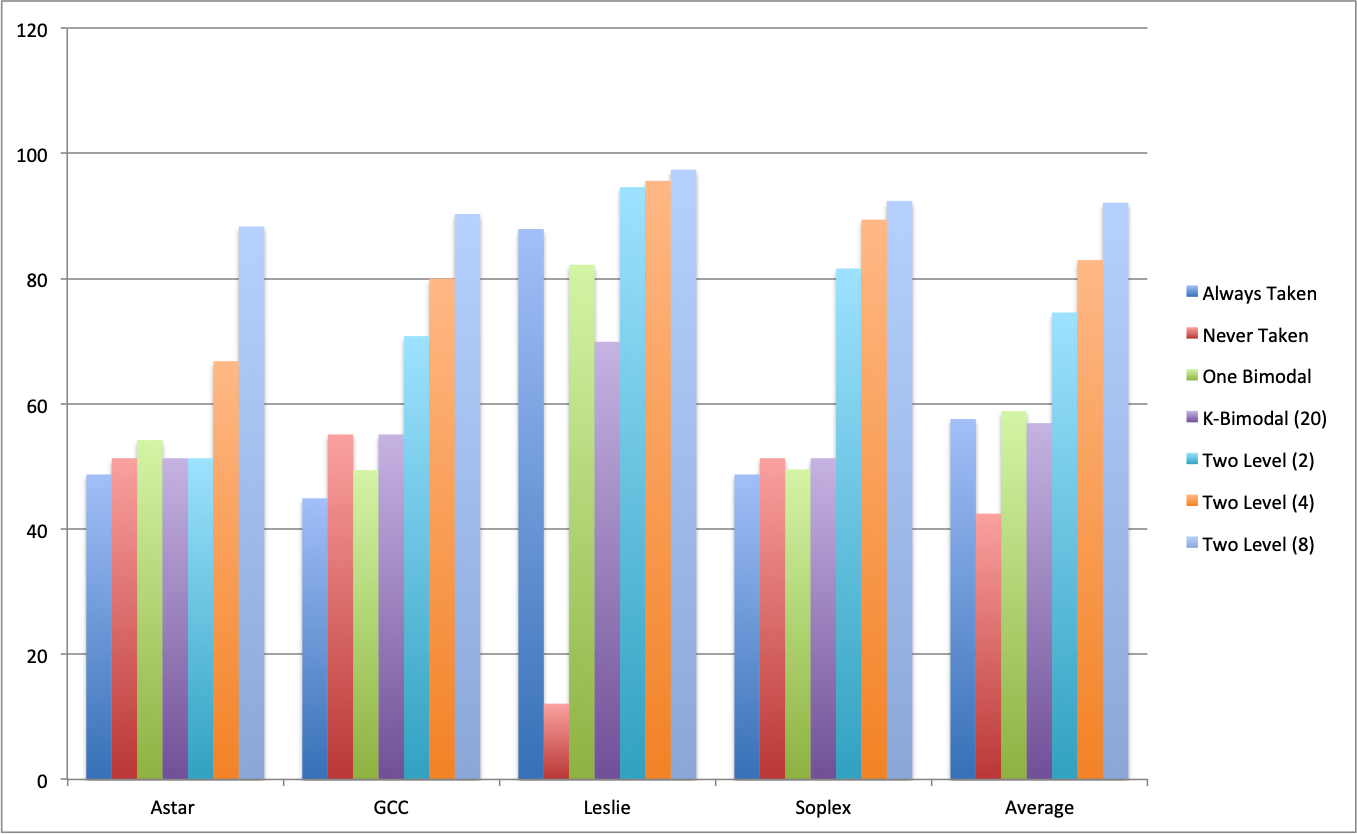
\includegraphics[height=.45\textheight]{accuracy.png}
  \caption{Branch Predictor Accuracy.}
\end{figure}

\begin{figure}[t]
  \centering
  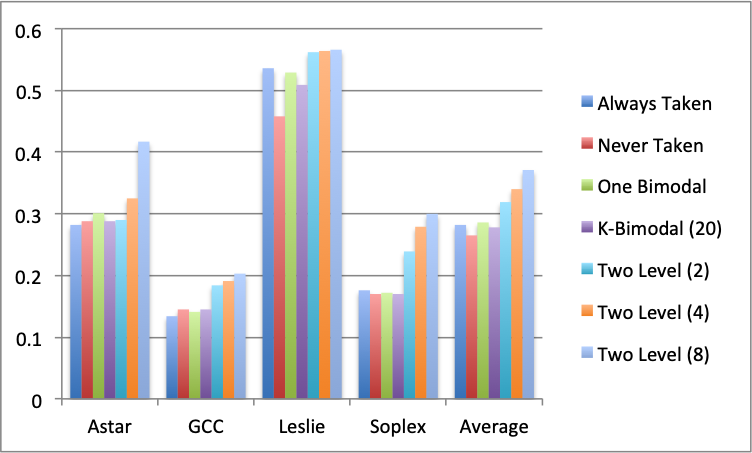
\includegraphics[height=.45\textheight]{ipc.png}
  \caption{Branch Predictor Accuracy.}
\end{figure}


\end{document}